\chapter{Esempio d'utilizzo}
    In questo capitolo illustro l'intero processo di progettazione del linguaggio, la creazione delle palette di simboli con DrawSE, la progettazione del diagramma e i risultati ottenuti dall'applicazione delle definizioni. Altro esempio d'utilizzo illustrato è quello in cui viene caricato un bundle di linguaggio\footnote{Insieme composto dal file della libreria di drawSE e dai file delle definizioni sintattiche e semantiche.} dal server.

    \section{Bundle di Linguaggio}
        Per caricare un bundle di linguaggio dal server inserisco all'interno dell'URL come parametri \texttt{loadLanguage} e il nome del bundle da caricare come valore del parametro. Ad esempio, inserendo il parametro \texttt{loadLanguage=er} verrà il caricato il bundle del liguaggio dalla cartella \textit{EXAMPLES/er}. All'interno della cartella \textit{er} devono essere presenti i seguenti file:
        \begin{itemize}
            \item \textit{library.xml} è la libreria dei simboli esportata con drawSE;
            \item \textit{newDefinition.json} è file JSON contenente la definizione sintattica del linguaggio;
            \item \textit{newSemanticDefinition.json} è il file JSON contenente la definizione semantica del linguaggio.
        \end{itemize}.
        \textit{EXAMPLES} risiede all'interno della directory principale di TiveJS.

    \section{Entity Relationship}
        Nello specifico, illustro la creazione del linguaggio Entitiy Relationship.

        \subsection{Creazione Palette di simboli con DrawSE}
            Il set di simboli che andrò ad utilizzare per la progettazione del diagramma viene creato attraverso l'usilio di drawSE, piattaforma descritta all'interno del capitolo 2, sezione 3. In questo esempio creo i simboli che poi andrò ad inserire all'interno di una palette che utilizzerò in TiveJS.
            \newline
            Lanciata l'applicazione, per creare un nuovo simbolo utilizzo quelli messi a disposizione da drawSE trascinando uno di questi all'interno dell'area di lavoro (foglio principale). A questo punto ho a disposizione due modalità di modifica del simbolo, \textit{Shape Mode} e \textit{AP Mode}. Con la prima definisco l'aspetto grafico del simbolo e con la seconda le posizione dei punti d'attacco. Personalizzato l'aspetto grafico del simbolo decido quali devono essere i suoi punti d'attacco.
            \newline
            Per creare una nuova palette clicco sul bottone \textit{New Palette} all'interno della barra laterale sinistra e trascino al suo interno i simboli dall'area di lavoro. A questo punto l'applicazione chiede che nome dare al simbolo trascinato (il nome deve essere unico).

        \subsection{Progettazione Diagramma}
            TiveJS mi permette di importare la libreria creata con drawSE cliccando su \textit{File -> Open Library from -> Device...} Una volta importata comparirà nella barra laterale sinistra come mostrato in figura \ref{fig:library}.
            \begin{figure}[htbp]
                \centering
                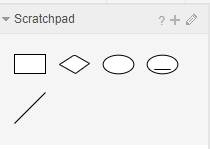
\includegraphics[scale=0.6]{Figure/drawse/library.PNG}
                \caption{Palette di simboli creata con DrawSE}
                \label{fig:library}
            \end{figure}
            Trascinando i simboli all'interno dell'area di lavoro compongo la sentenza visiva ottenendo un diagramma come mostrato in figura \ref{fig:sentence}.
            \begin{figure}[htbp]
                \centering
                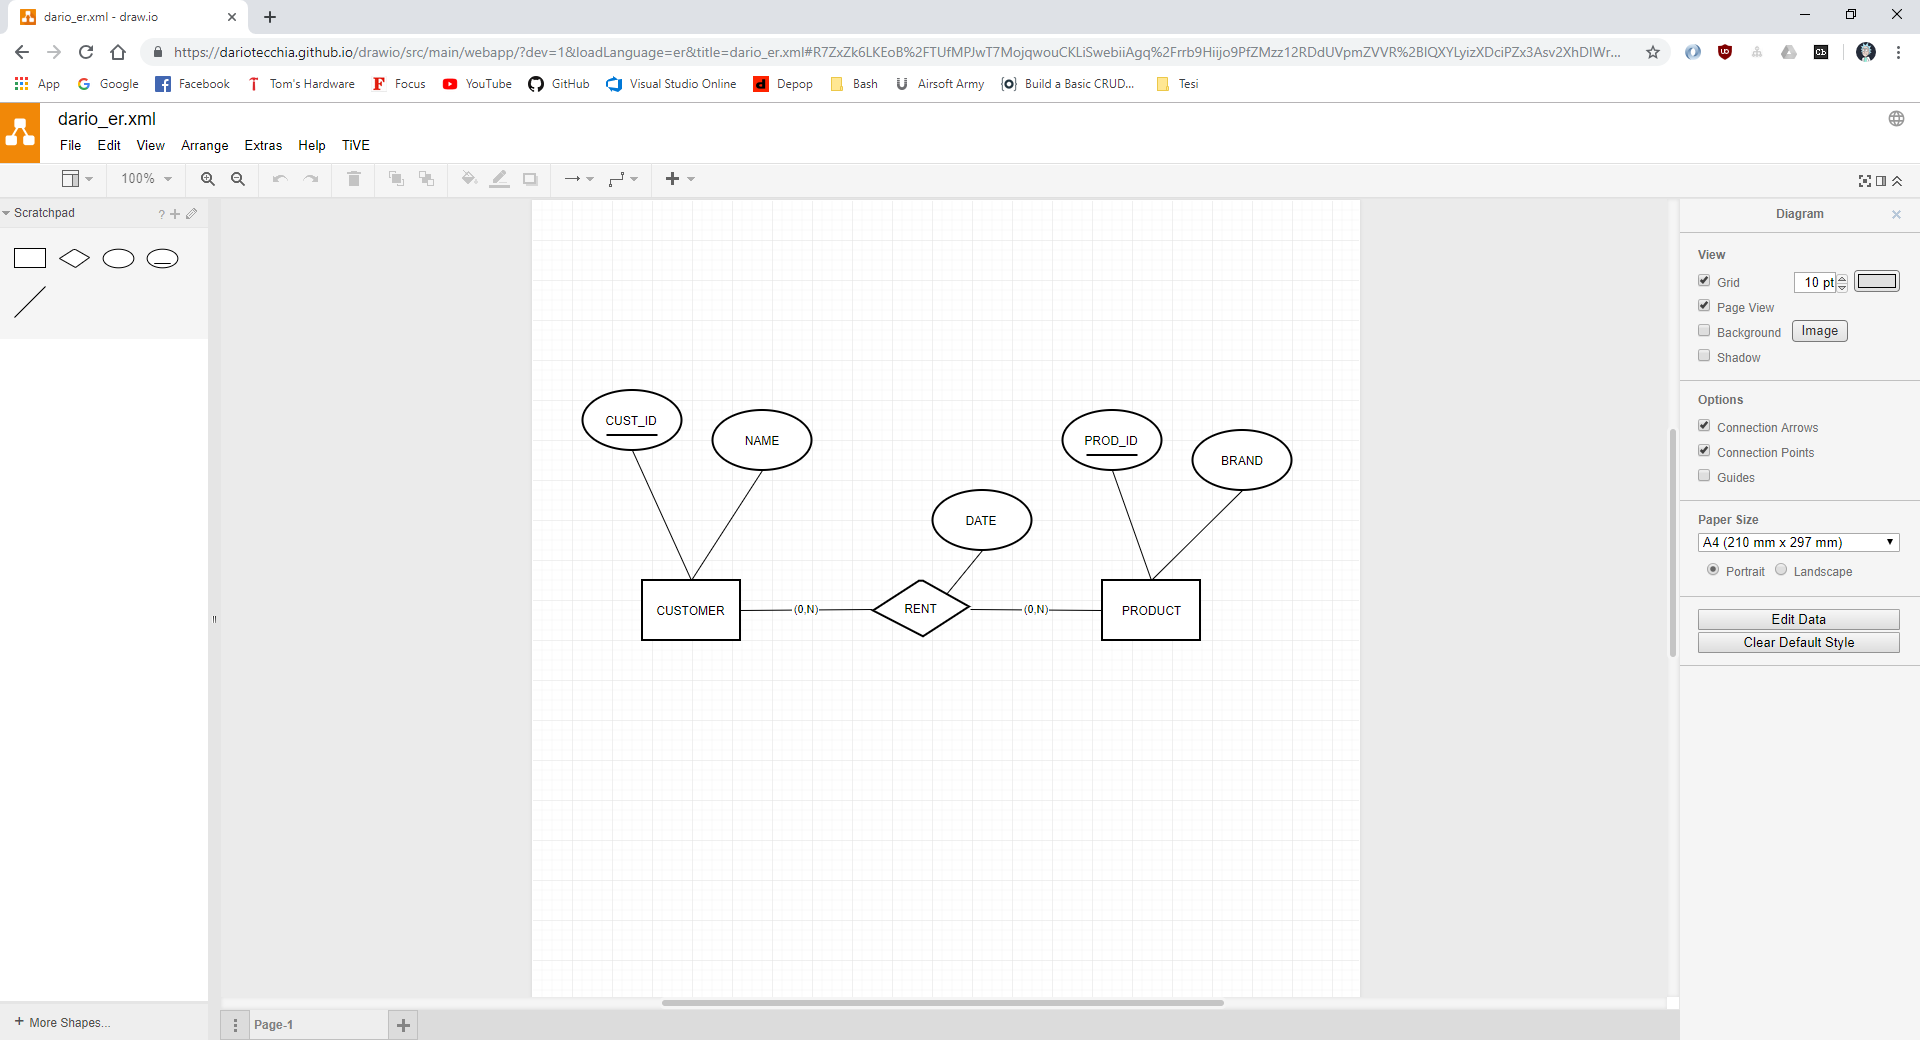
\includegraphics[scale=0.25]{Figure/drawse/sentence.PNG}
                \caption{Diagramma ER}
                \label{fig:sentence}
            \end{figure}

        \subsection{Definizione Linguaggio}
            Una delle fasi principali della creazione di un linguaggio sono la definizione delle specifiche sintattiche e semantiche che quest'ultimo dovrà rispettare.
            \newline
            La specifica sintattica si preoccupa di come deve essere la struttura del grafo e le regole che ogni componente al suo interno deve rispettare. La specifica semantica raffina la definizione sintattica e la estende creando uno schema di traduzione del grafo.

            \subsubsection{Creazione Definizioni Sintattiche}
                La definizione della specifica sintattica del linguaggio avviene creando un file JSON che rispetti la struttura illustrata nell'appendice \ref{appendix:syntaxSchema}. Il risultato è mostrato nell'appendice \ref{appendix:erSyntaxDefinition}.

            \subsubsection{Creazione Definizioni Semantiche}
                Come per quella sintattica, la specifica semantica viene definita attraverso un file JSON che rispetti lo schema illustrato nell'appendice \ref{appendix:semanticSchema}. Il risultato è mostrato nell'appendice \ref{appendix:erSemanticDefinition}.

        \subsection{Caricamento e Applicazione Definizioni}
            Create le definizioni procedo con il caricamento di quest'ultime sulla piattaforma attraverso l'apposito menu illustrato in figura \ref{fig:tivemenu}.

            \subsubsection{Sintattiche}
                Le definizioni sintattiche le carico cliccando su \textit{TiVE -> Load Rules...} e le applico su un diagramma cliccando su \textit{TiVE -> Apply Rules}
                \newline
                Se tutte le regole vengono rispettate otterrò il risultato mostrato in figura \ref{fig:syntaxOK}.
                \begin{figure}[htbp]
                    \centering
                    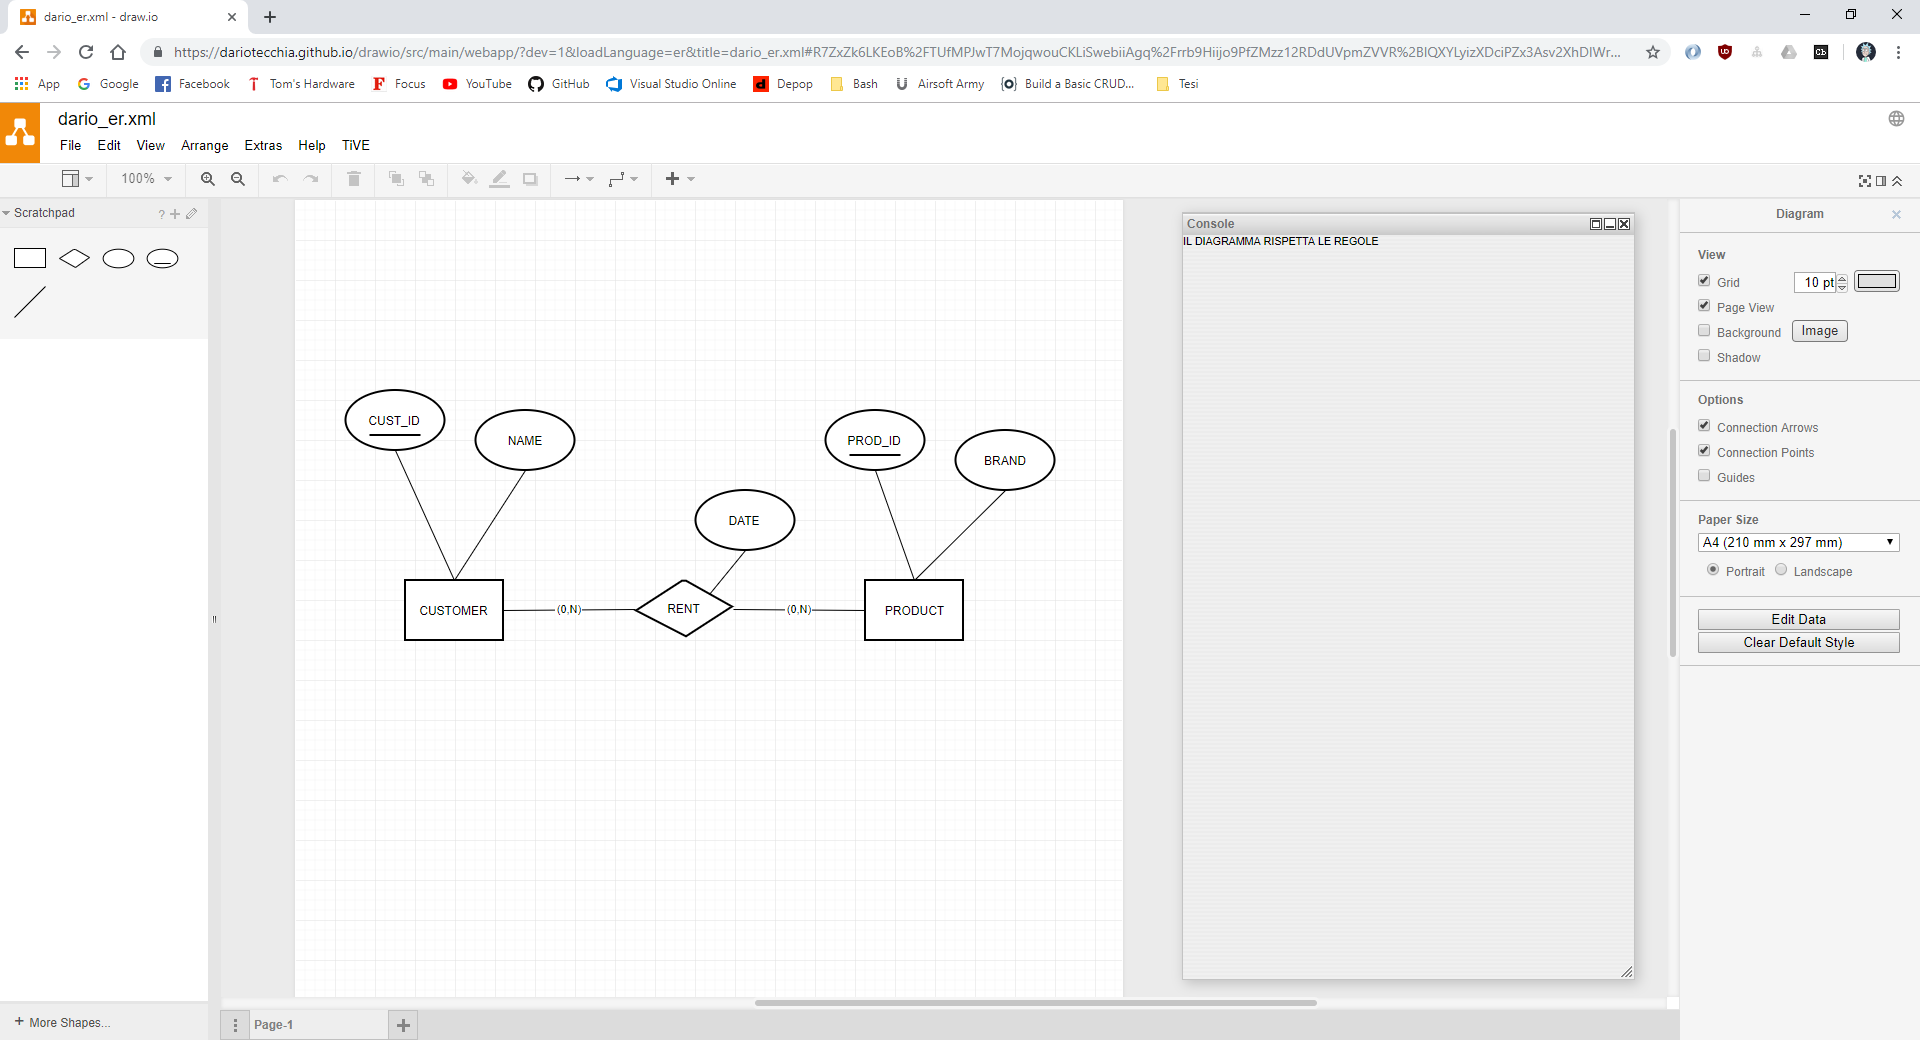
\includegraphics[scale=0.25]{Figure/drawse/syntax_rule_OK.PNG}
                    \caption{Applicazione delle definizioni sintattiche avvenuta con successo}
                    \label{fig:syntaxOK}
                \end{figure}
                \newline
                Altrimenti otterrò il risultato mostrato in figura \ref{fig:syntaxNO}.
                \begin{figure}[htbp]
                    \centering
                    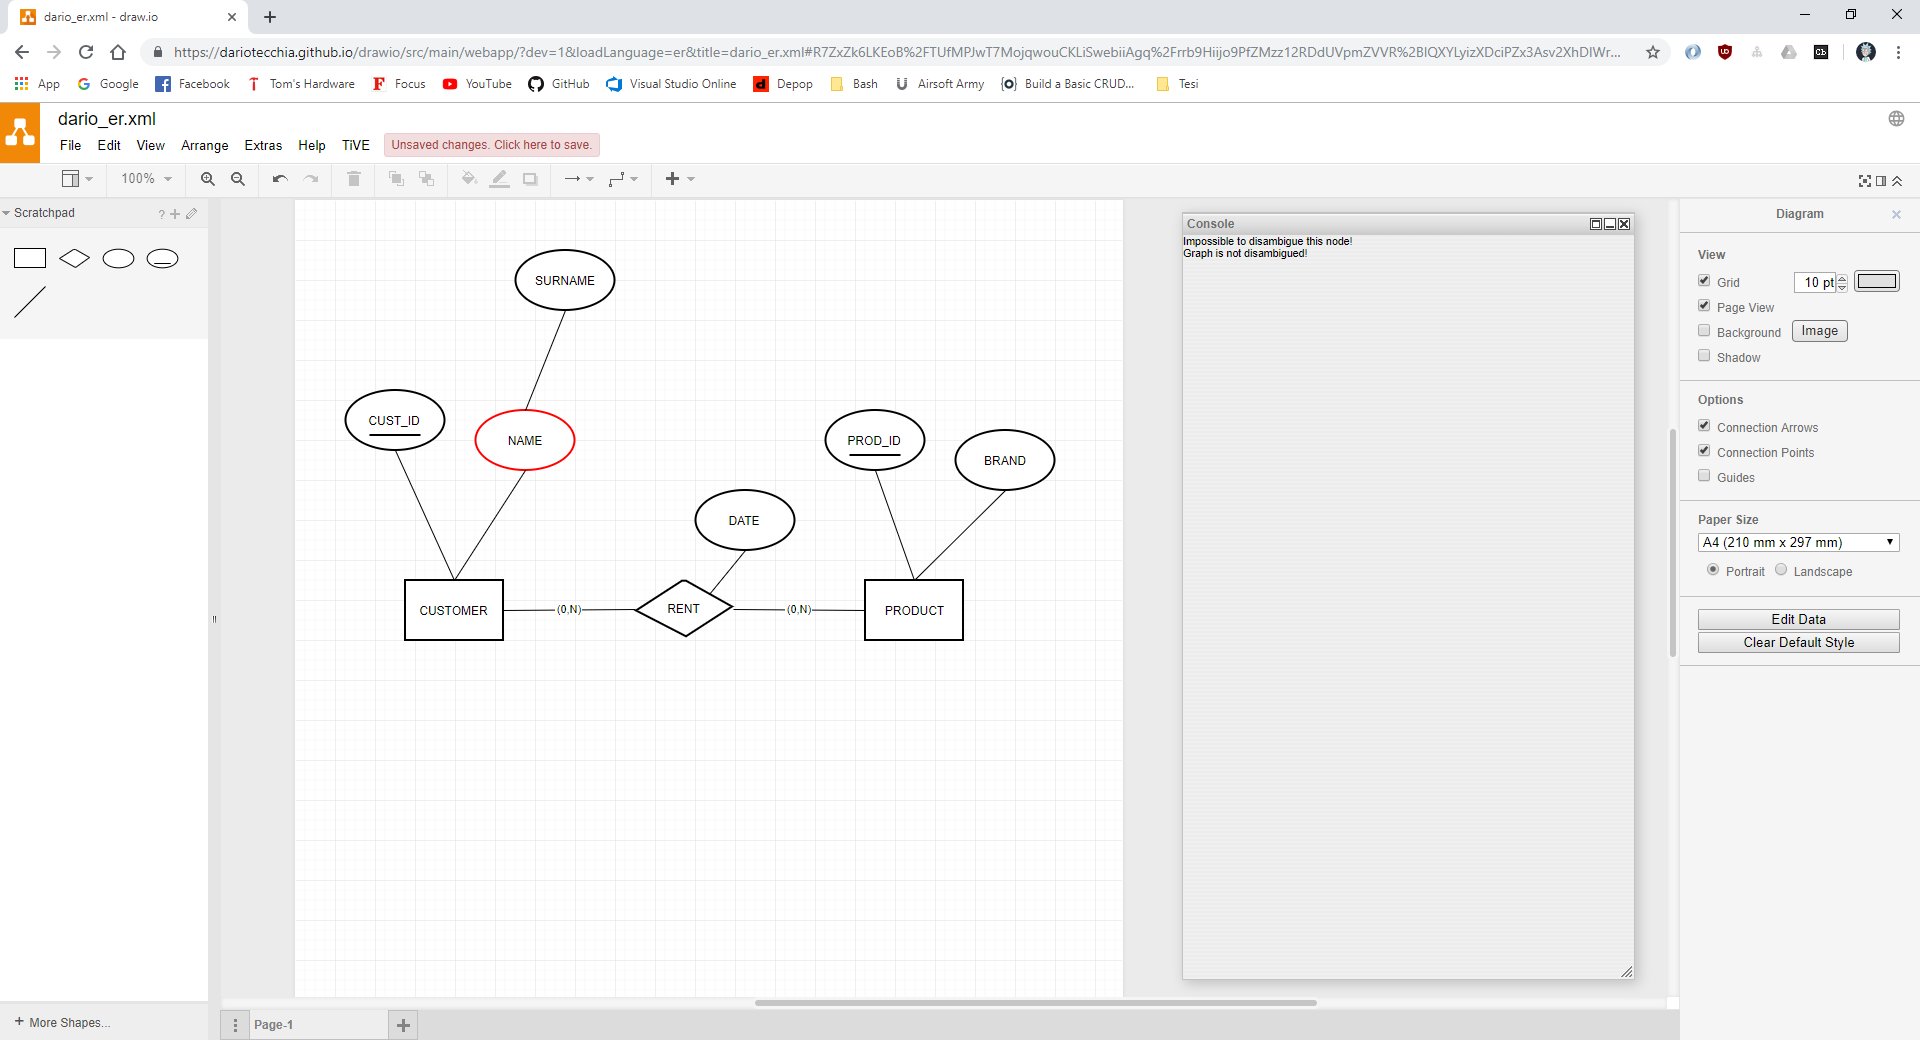
\includegraphics[scale=0.25]{Figure/drawse/syntax_rule_FAIL.PNG}
                    \caption{Applicazione delle definizioni sintattiche fallita}
                    \label{fig:syntaxNO}
                \end{figure}
                \newline
                Le definizioni sintattiche possono essere applicate e prescindere dalla presenza delle definizioni semantiche.

            \subsubsection{Semantiche}
                Le definizioni semantiche le carico cliccando su  \textit{TiVE -> Load Semantic Rules...} e come per le definizioni sintattiche, le applico cliccando su \textit{TiVE -> Apply Rules}.
                \newline
                Se il controllo sintattico va a buon fine l'algoritmo passa alla valutazione delle regole semantiche. Se tutto va a buon fine ottengo la traduzione semantica del diagramma, come mostrato in figura \ref{fig:semanticOK}
                \begin{figure}[htbp]
                    \centering
                    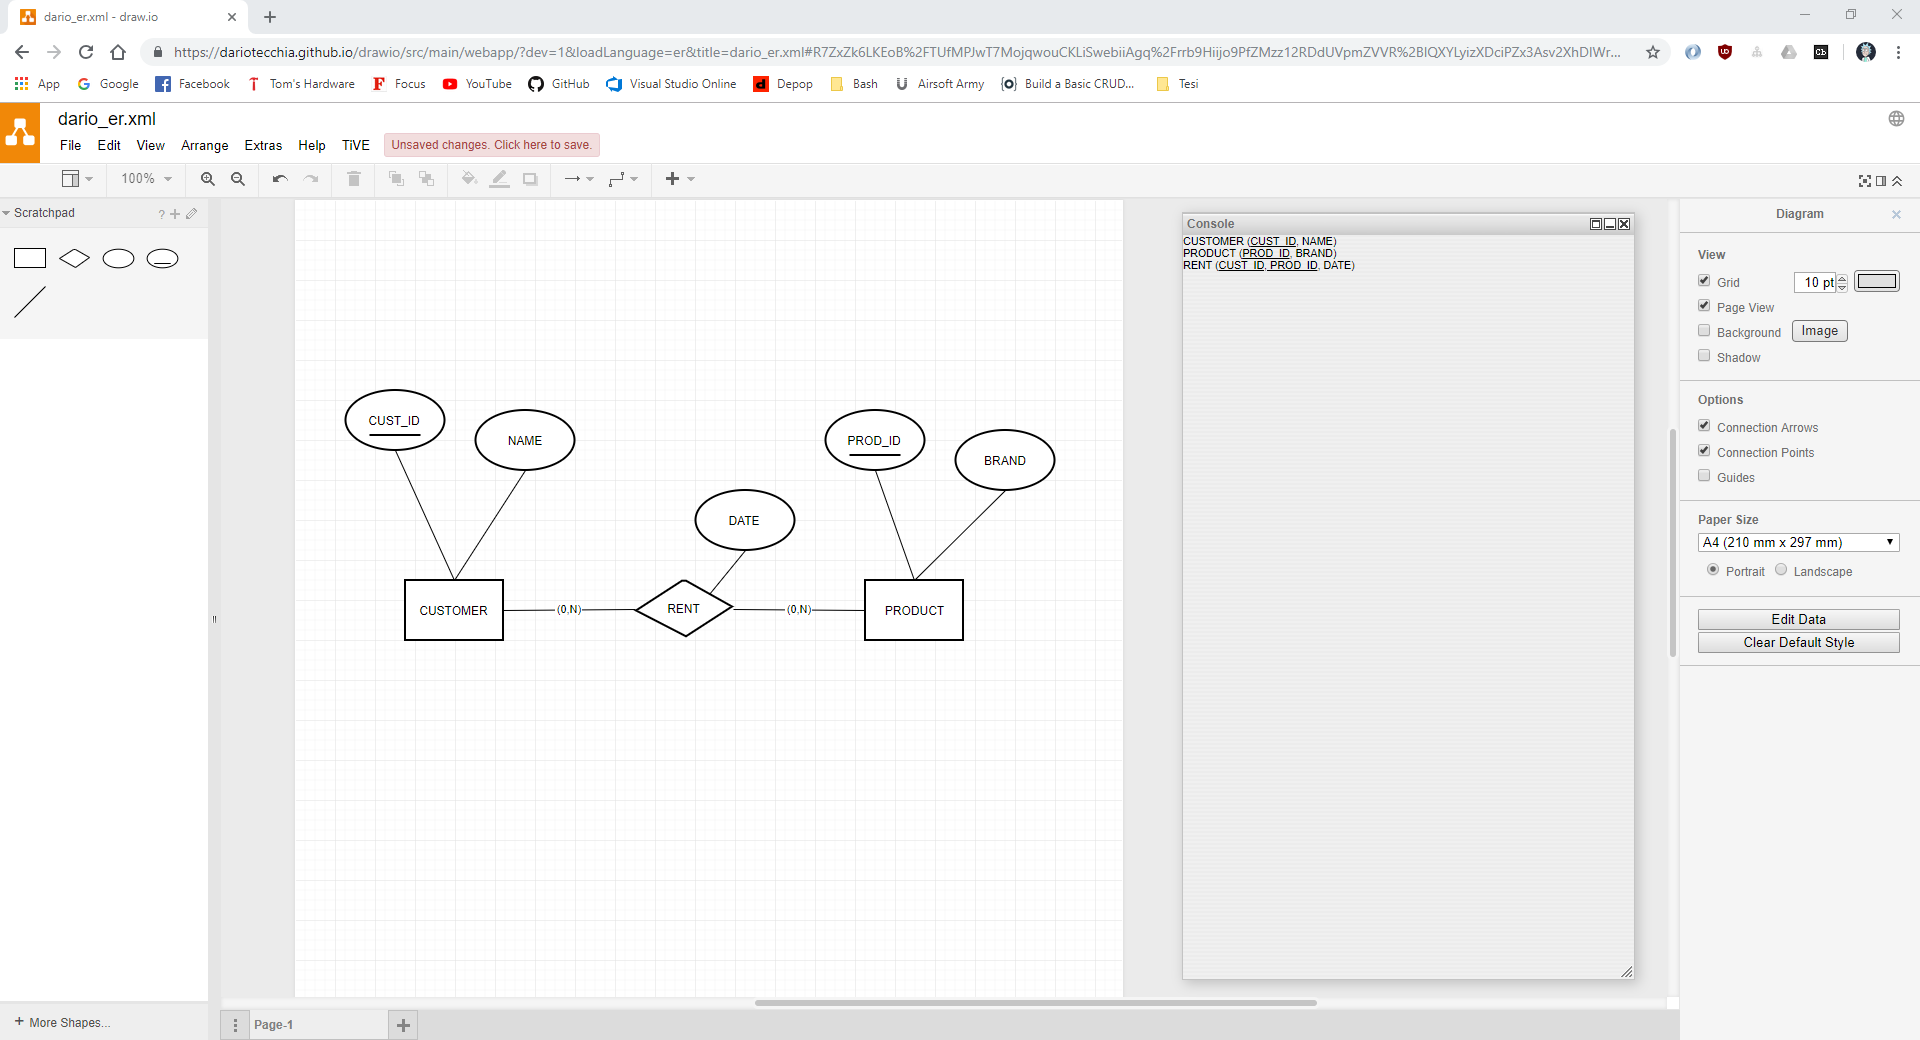
\includegraphics[scale=0.25]{Figure/drawse/semanticOK.PNG}
                    \caption{Applicazione delle definizioni semantiche avvenuta con successo}
                    \label{fig:semanticOK}
                \end{figure}